\chapter{Sequenzdiagramme}

\section{Import von einem JOANA Graphen(Pflichtenheft 9 /T010/)}

\begin{figure}[hb]
  \centering
  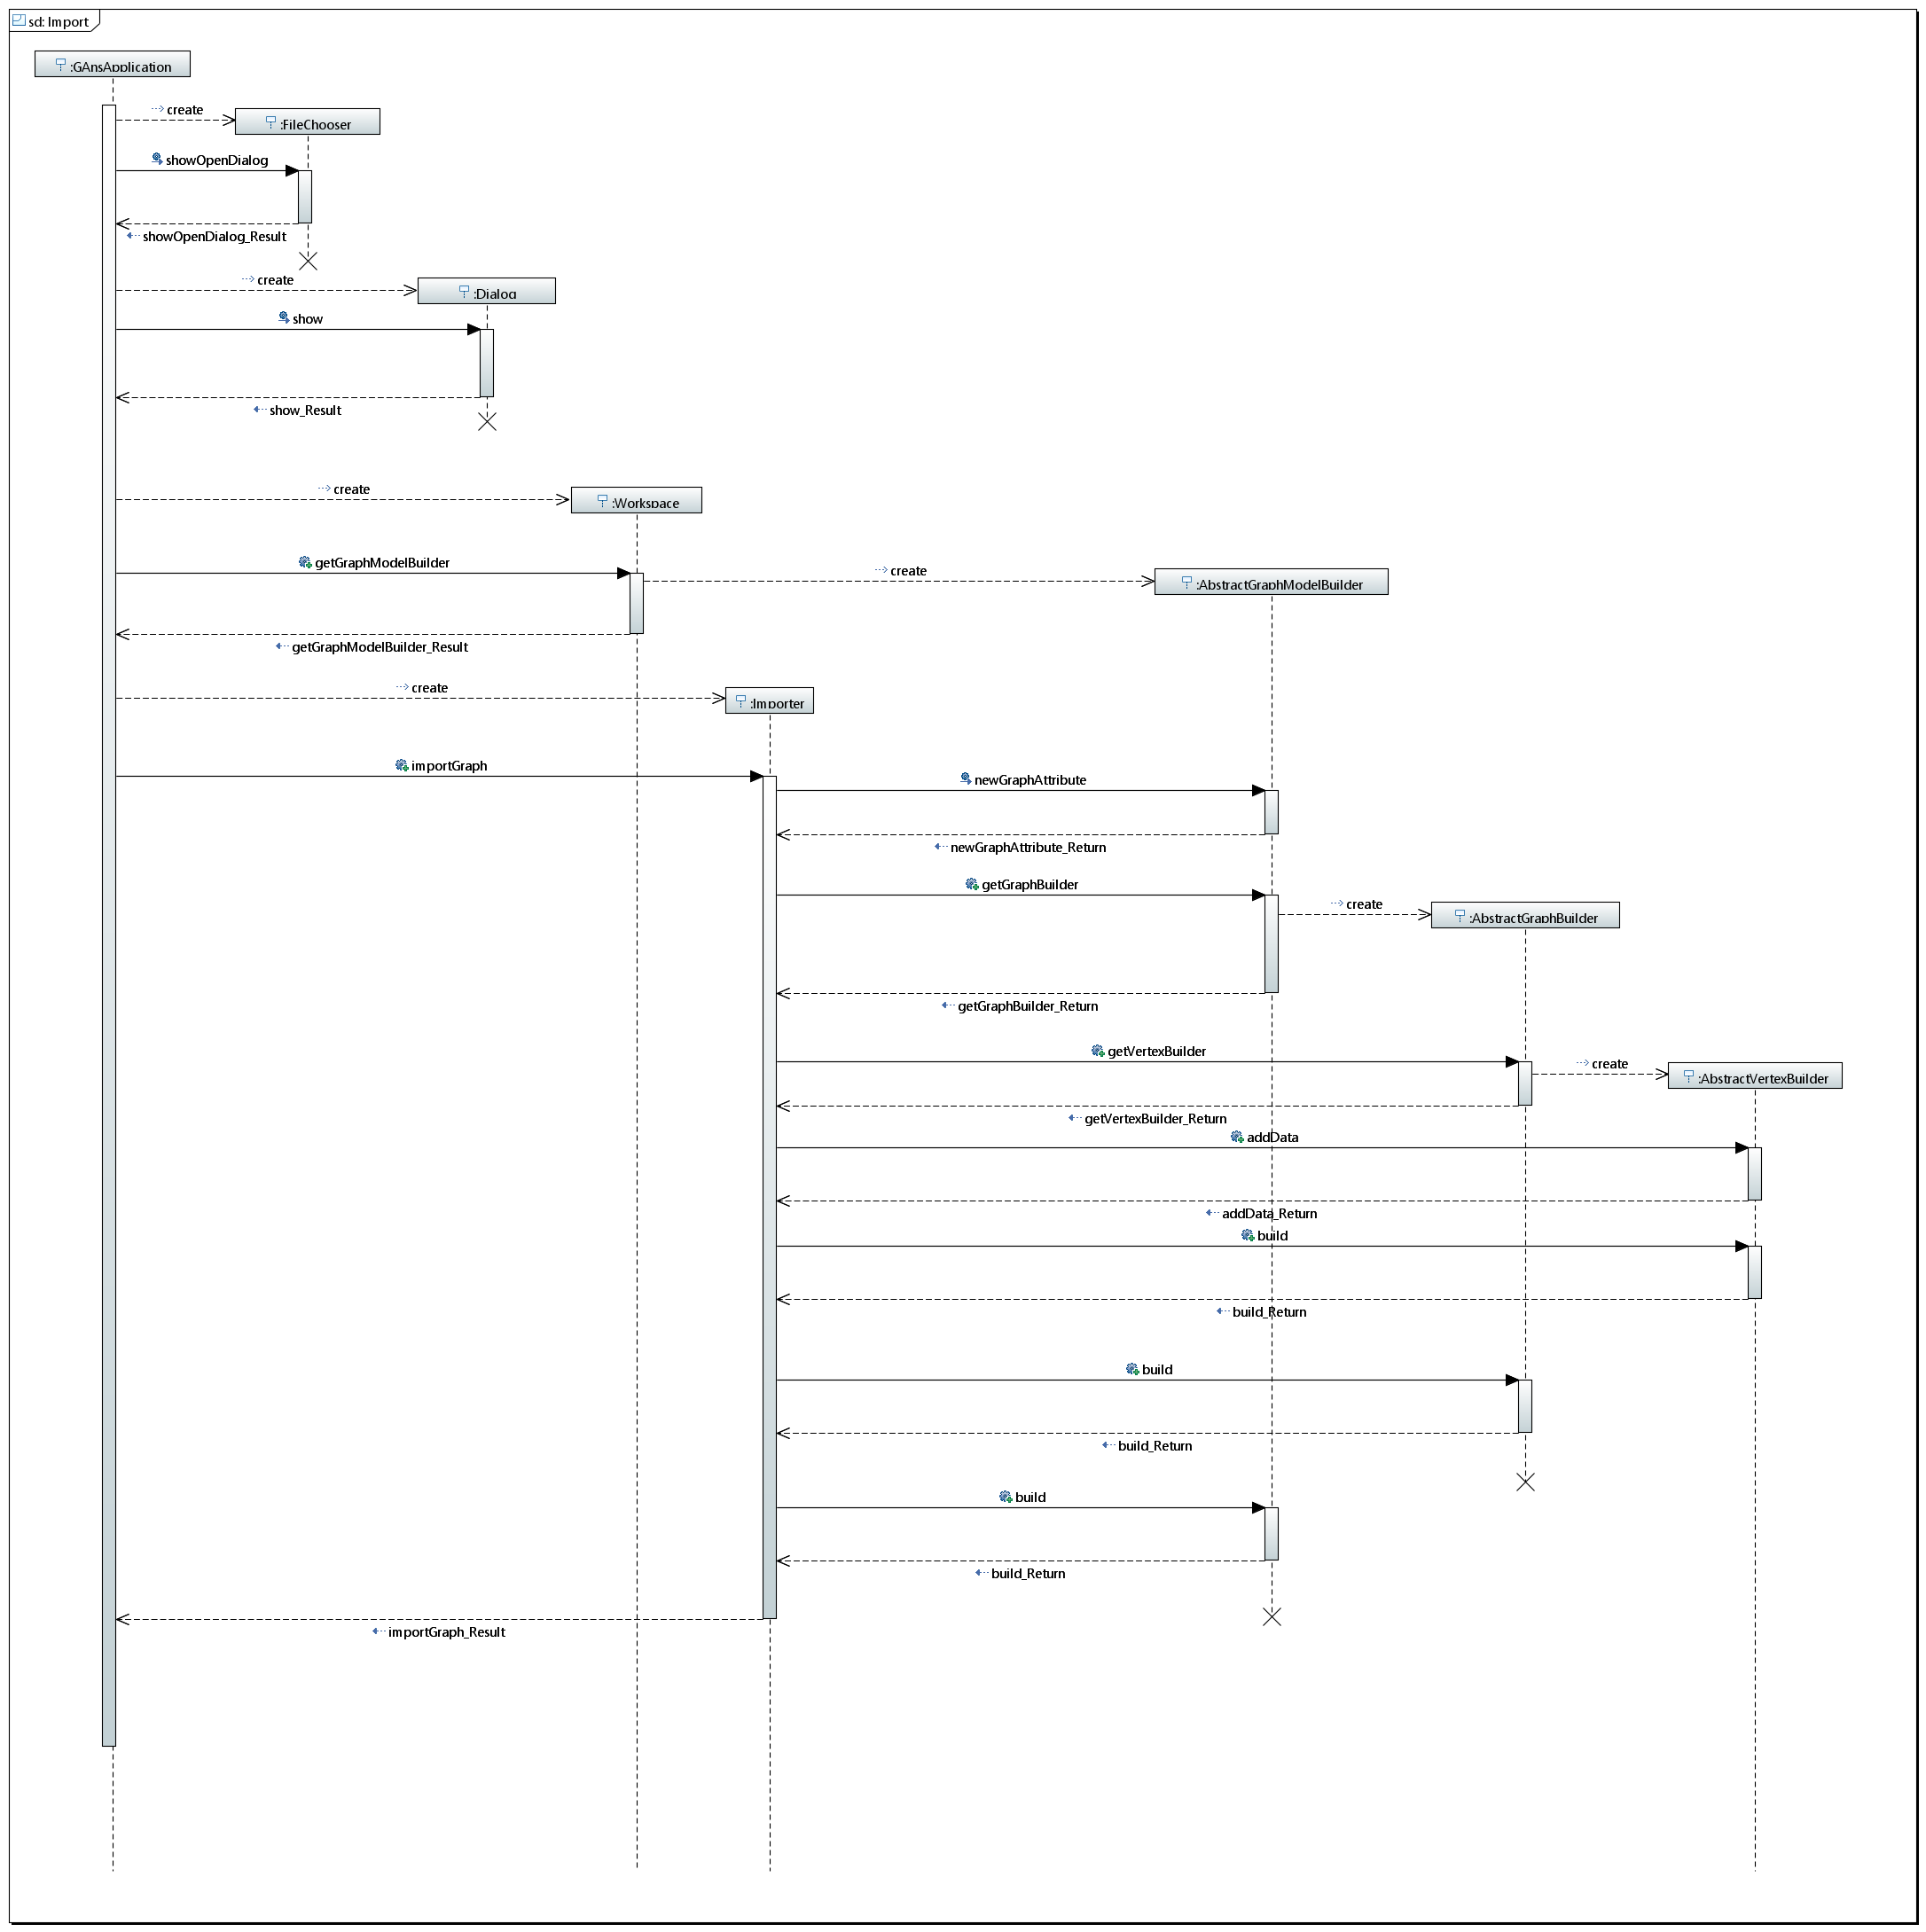
\includegraphics[width=380pt]{resourcen/SeqDiagramImport.PNG}
  \caption{Sequenz Diagramm für den Import}
  \label{fig:gui_view_treeview}
\end{figure}

Der Benutzer möchte einen Graphen importieren und klickt auf Import. Die GAnsApplication öffnet einen FileChooser, in welchem der Benutzer die Datei auswählen will welche er implementieren möchte. Danach öffnet sich ein Workspace Dialog in welchem der Benutzer auswählt von welchem Typ der Graph ist.\\
Das Workspace übergibt der GAnsApplication nun den dazugehörigen AbstractGraphModelBuilder. Dieser wird dann dem Importer übergeben, welcher mithilfe des Builders eine Repräsentation des Graphen zurückgibt welcher auf den Workspace spezifiziert ist.

\section{Öffnen eines JOANA-Methodengraphen (Pflichtenheft 9 /T020/)}

\section{Selektieren mehrerer Knoten und Kanten (Pflichtenheft 9 /T030/)}

\section{Navigation (Pflichtenheft 9 /T040/)}

\section{Constraint zu Knoten eines geladenen Graphen hinzufügen (Pflichtenheft 9 /T050/)}

\section{Filtern von Kanten (Pflichtenheft 9 /T060/)}

\section{Export von einem geladenen JOANA-Graphen als SVG (Pflichtenheft 9 /T070/)}